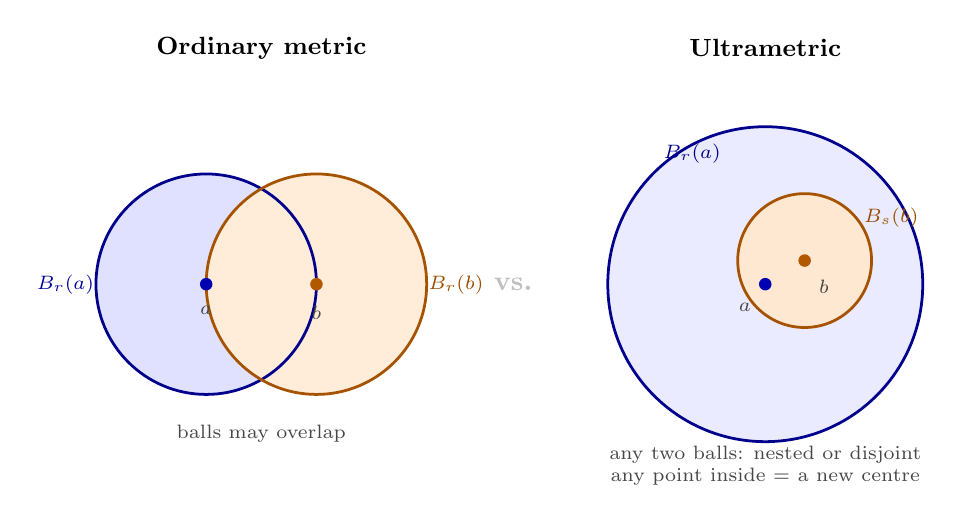
\begin{tikzpicture}[
  dot/.style={circle,fill,inner sep=1.6pt},
  lbl/.style={font=\small},
  sublbl/.style={font=\scriptsize,text=gray!55!black}
]

% ---- LEFT: Ordinary metric — balls can overlap ----
\begin{scope}[shift={(-3.2,0)}]
  \node[lbl,font=\small\bfseries] at (0,3.0) {Ordinary metric};

  % Two overlapping balls
  \fill[blue!12] (-0.7,0) circle (1.4cm);
  \fill[orange!15] (0.7,0) circle (1.4cm);
  \draw[blue!55!black, line width=1.0pt] (-0.7,0) circle (1.4cm);
  \draw[orange!65!black, line width=1.0pt] (0.7,0) circle (1.4cm);

  \node[dot,fill=blue!70!black] at (-0.7,0) {};
  \node[dot,fill=orange!70!black] at (0.7,0) {};
  \node[sublbl,anchor=north] at (-0.7,-0.15) {$a$};
  \node[sublbl,anchor=north] at (0.7,-0.15)  {$b$};
  \node[sublbl,text=blue!60!black,anchor=east] at (-2.0,0) {$B_r(a)$};
  \node[sublbl,text=orange!60!black,anchor=west] at (2.0,0) {$B_r(b)$};

  % Overlap label
  \node[sublbl,align=center] at (0,-1.9) {balls may overlap};
\end{scope}

% ---- RIGHT: Ultrametric — balls are nested or disjoint ----
\begin{scope}[shift={(3.2,0)}]
  \node[lbl,font=\small\bfseries] at (0,3.0) {Ultrametric};

  % Outer ball
  \fill[blue!8] (0,0) circle (2.0cm);
  \draw[blue!55!black, line width=1.0pt] (0,0) circle (2.0cm);

  % Inner ball (nested inside outer)
  \fill[orange!18] (0.5,0.3) circle (0.85cm);
  \draw[orange!65!black, line width=1.0pt] (0.5,0.3) circle (0.85cm);

  \node[dot,fill=blue!70!black] at (0,0) {};
  \node[dot,fill=orange!70!black] at (0.5,0.3) {};
  \node[sublbl,anchor=north east] at (-0.06,-0.12) {$a$};
  \node[sublbl,anchor=north west] at (0.56,0.18) {$b$};
  \node[sublbl,text=blue!55!black,anchor=south west] at ({-2.0*0.707},{2.0*0.707}) {$B_r(a)$};
  \node[sublbl,text=orange!60!black] at (1.6,0.85) {$B_s(b)$};

  % Key property annotation
  \node[sublbl,align=center] at (0,-2.3)
    {any two balls: nested or disjoint\\
     any point inside = a new centre};
\end{scope}

% Divider label
\node[lbl,text=gray!50,font=\normalsize\bfseries] at (0,0) {vs.};

\end{tikzpicture}